\chapter{Qualité Logicielle}
\minitoc

Ce chapitre détaille les aspects de qualité logicielle qui ont été pris en compte tout le long du projet.

\section{Un projet conséquent}

Cette application a nécessité un travail assez conséquent~:

\begin{itemize}
\item 170 Révisions
\item 3640 lignes de code
\end{itemize}

Pour produire un travail maintenable, efficace et fonctionnel, ces nombreuses lignes de code ont du être 
écrite en respectant certaines règles. En effet, nous avons utilisé l'outil checkstyle qui permet de produire un code qui respecte toujours la même syntaxe même si nous sommes plusieurs développeurs.

\section{Utilisation de Sonar}
Sonar est outil qui s'inscrit parfaitement dans cette démarche. En effet, il analyse le code et produit un rapport de statistiques selon plusieurs critères.

\begin{figure}[!h]
 \centering
 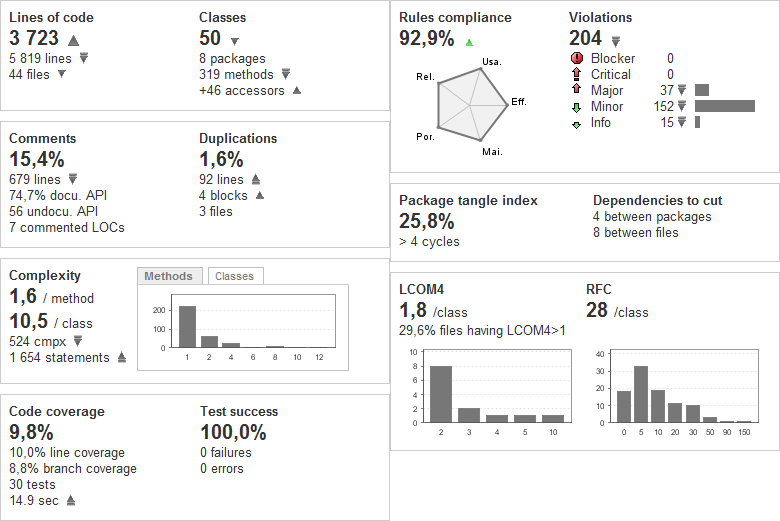
\includegraphics[width=16cm]{images/sonar-dashboard.png} 
 \caption{Tableau de bord de Sonar}
 \label{fig:sonar-dashboard}
\end{figure}

La capture de la figure~\ref{fig:sonar-dashboard} présente le tableau de bord que produit Sonar pour notre projet. Les critères a analyser sont les suivants~:

\begin{itemize}
\item Nombres de lignes de codes, de classes, etc.
\item Respect des règles syntaxiques
	\begin{itemize}
	\item Efficacité
	\item Maintenabilité
	\item Portabilité
	\item Fiabilité
	\item Utilisabilité
	\end{itemize}
\item Complexité
\item Documentation
\item Couverture de tests
\end{itemize}


Les statistiques de Sonar ont permis de développer en suivant les axes de qualité que Sonar analyse. Cela nous a ainsi permis de produire du code propre. En effet, selon Sonar, le code du projet Alma Speech Recognition respecte les critères présentés par la figure~\ref{fig:sonar-axes}

\begin{figure}[!h]
 \centering
 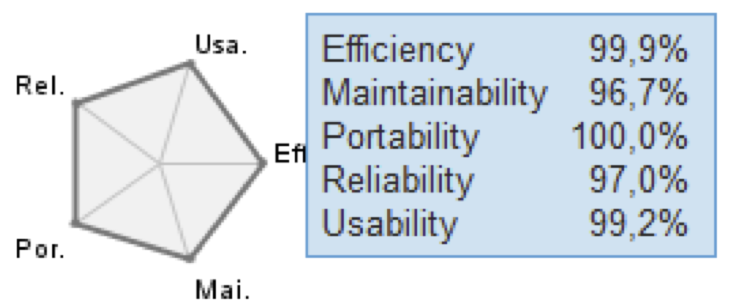
\includegraphics[scale=1]{images/sonar-axes.png} 
 \caption{Axes de qualité de Sonar}
 \label{fig:sonar-axes}
\end{figure}

Ce graphique nous montre les résultats de l'analyse du code par Sonar. On remarque que le code respecte à plus de environ 97\% les différents critères. Cet outil s'est donc avéré très efficace durant de développement.

De plus, les courbes de progression de Sonar nous montrent que le respect de ces critères n'a cessé d'augmenter au fur et à mesure de l'avancement.



